\documentclass[twocolumn,10pt]{article}
\usepackage[letterpaper,left=1.95cm,right=1.95cm,top=2.5cm,bottom=3.16cm]{geometry}
\usepackage{natbib}
\usepackage{hyperref}
\usepackage{amsmath,amssymb}
\usepackage[utf8]{inputenc}
\usepackage{pxfonts}
\usepackage{wasysym}
\usepackage{amssymb}
\usepackage{abstract}
\usepackage{parskip}
\usepackage{hyperref}
\usepackage{titlesec}
\usepackage{xcolor}
\usepackage{natbib}

\hypersetup{
    colorlinks=false,
    linkbordercolor={white},
    citebordercolor={white}
}
\usepackage{float}
\usepackage{graphicx}
\usepackage{fancyhdr}
\usepackage{titling}
\usepackage{caption}
\captionsetup[table]{
  position=above,
  justification=raggedright,
  labelsep=newline,
  singlelinecheck=false
}
\usepackage[document]{ragged2e}
\usepackage[affil-sl]{authblk}
\usepackage{mathptmx}
\usepackage{microtype}

\setlength{\columnsep}{1cm}
\emergencystretch=2em
\renewcommand{\refname}{BIBLIOGRAFÍA}
\renewcommand{\figurename}{Fig.}
\renewcommand{\tablename}{Tabla.}
\renewcommand{\abstractname}{RESUMEN}

\providecommand{\keywordsSpan}[1]{
  \small
  \textbf{\textit{Palabras Clave:}} #1
}

\providecommand{\keywordsEng}[1]{
  \small
  \textbf{\textit{Keywords:}} #1
}

\titleformat{\section}
  {\normalfont\large\bfseries}{\makebox[30pt][l]{\thesection}}{0pt}{}
\titleformat{\subsection}
  {\normalfont\large\bfseries}{\makebox[30pt][l]{\thesubsection}}{0pt}{}
\renewcommand\thesection{\arabic{section}.}
\renewcommand\thesubsection{\thesection\arabic{subsection}}

\makeatletter
\long\def\@makecaption#1#2{
\vskip\abovecaptionskip
\sbox\@tempboxa{#1. #2}
\ifdim \wd\@tempboxa >\hsize
#1. #2\par
\else
\global \@minipagefalse
\hb@xt@\hsize{\hfil\box\@tempboxa\hfil}
\fi
\vskip\belowcaptionskip}
\makeatother

\pagestyle{fancyplain}
\fancyfoot[C]{}
\renewcommand\plainheadrulewidth{.4pt}
\rhead{Semestre 4 Año 2026, Grupo X, páginas XX-XX}
\lhead{Estadística Bayesiana}
\rfoot{\thepage}

\fancypagestyle{alim}{%
  \fancyhf{}
  \renewcommand{\headrulewidth}{0pt}
  \rfoot{\thepage}
}

\date{}


{\title{\fontsize{16}{16}
\vspace*{-0.7cm}
\textbf{Variación mensual de las ventas de muebles y artículos del hogar: una referencia para el inventario}\\[0.2cm]
\fontsize{12}{12}
\textbf{Monthly Variation in Furniture and Home Furnishings Sales: A Reference for Inventory}\\[0.2cm]}
}

\author[1,*]{\fontsize{10pt}{10pt}\selectfont\textbf{Juan Esteban Jiménez Aristizábal}}
\author[1]{\textbf{David Quijano}}
\author[1]{\textbf{Juan Esteban Zambrano}}
\author[1]{\textbf{Juan Angel Triana Olarte}}

\affil[1]{\fontsize{8pt}{8pt}\selectfont Pregrado Ciencia de Datos Universidad Externado, Bogotá - Colombia}
\affil[*]{\fontsize{8pt}{8pt}\selectfont
juan.jimenez28@est.uexternado.edu.co\\
david.quijano@est.uexternado.edu.co\\
juan.zambrano4@est.uexternado.edu.co\\
juan.triana2@est.uexternado.edu.co}

\begin{document}
\twocolumn[
  \maketitle
  \begin{abstract}
\justifying
Quien decide cuánto inventario mantener casi siempre trabaja con una sola cifra de ventas esperadas, pero lo que más pesa es qué tan lejos puede quedar la demanda real. En este trabajo medimos esa distancia para las ventas de muebles y artículos del hogar en Estados Unidos, con datos mensuales de FRED \citep{fred2026} entre marzo de 1992 y julio de 2026. Usamos un modelo bayesiano de regresión con errores \textit{t} de Student, factores por mes en marzo--junio de 2020 y un parámetro de mayor volatilidad desde julio de 2020, conservando los meses extremos en lugar de eliminarlos. Las ventas de electrónica, construcción y tiendas generales se mueven junto con las de muebles, pero explican poca variación: el modelo no acierta mejor la cifra mensual que la media histórica (RMSE 2.04 frente a 2.02 en 24 meses de prueba). Aun así, el intervalo predictivo del 90\% cubrió el valor observado en 23 de 24 meses y fue más angosto que una alternativa sin factores de pandemia (ancho medio 6.9 frente a 9.5 puntos de crecimiento). Para agosto de 2026 estimamos ventas entre 10\,134 y 11\,050 millones de dólares al 90\%, frente a 10\,537 en julio. Concluimos que el aporte útil es el \textbf{rango de incertidumbre} macro para inventario: la comercializadora lo escala a su volumen (participación o factor histórico frente al sector) para fijar techo, piso e inventario de seguridad en compras, sin sustituir su pronóstico interno por SKU.
\end{abstract}
\keywordsSpan{inferencia bayesiana, ventas minoristas, inventario, incertidumbre, volatilidad}

\vspace{0.25cm}
\noindent\textbf{Abstract (English).}
\justifying
Inventory decisions often rely on a single expected sales figure; we quantify how far U.S.\ furniture and home furnishings demand may deviate using a Bayesian \textit{t}-regression with COVID scalers and post-2020 volatility. Point forecasts do not beat the historical mean (RMSE 2.04 vs.\ 2.02 on 24 hold-out months), but 90\% predictive intervals covered 23/24 months with narrower bands than a benchmark without pandemic factors. The deliverable is calibrated uncertainty for sector-level inventory planning (e.g.\ August 2026 sales: USD 10.1--11.0 billion at 90\%).

\keywordsEng{Bayesian inference, retail sales, inventory, uncertainty, volatility}

  \vspace{0.8em}
]
\thispagestyle{alim}

\section{INTRODUCCIÓN}
\justifying
Una comercializadora de artículos para el hogar decide periódicamente cuánto inventario mantener y cuánto pedir a proveedores. Para ello necesita anticipar cómo cambiará la demanda; equivocarse es costoso en ambos sentidos. Si se pide de menos, hay quiebres de stock y pérdida de clientes; si se pide de más, el capital queda inmovilizado en bodega y se asumen costos de almacenamiento y obsolescencia. En la práctica esa anticipación suele reducirse a \textbf{un solo número} (ventas esperadas del mes), aunque la realidad casi nunca coincide con él. Lo que fija el costo de decidir mal no es el error promedio sino \textbf{qué tan grande puede ser la desviación} respecto a esa cifra, y esa magnitud rara vez se comunica de forma explícita entre áreas.

Dentro de la empresa, compras, comercial y finanzas miran el mismo pronóstico con intereses distintos: compras evita desabastecimiento y exceso, comercial presiona por cumplir metas de venta y finanzas limita el efectivo en inventario. Sin una medida común de cuánto puede variar la \textbf{demanda del mercado}, cada área defiende un nivel de stock distinto a partir del mismo punto de partida. Este trabajo aporta esa referencia a nivel \textbf{macro} (sector estadounidense agregado), como paso previo y complemento a los pronósticos \textbf{micro} (empresa, categoría, SKU) que la firma ya maneja.

Antes de fijar pedidos a nivel producto hay que entender cómo se mueve el mercado en el que opera la firma. Usamos ventas minoristas mensuales de muebles y artículos para el hogar en Estados Unidos, estimadas por el Census Bureau y publicadas en FRED \citep{fred2026}. Son series desestacionalizadas, públicas y largas (mar.\ 1992--jul.\ 2026), aptas para medir variación normal, episodios extremos y cambios de volatilidad. No sustituyen el historial interno de la empresa, pero dan un \textbf{escenario sectorial} comparable entre compras, ventas y finanzas.

La respuesta del modelo es el crecimiento mensual $y_t = 100\cdot\Delta\log(\text{ventas}_t)$; las covariables capturan hipótesis de ciclo de consumo: otras categorías del comercio, ingreso disponible, presión de inventarios en el canal (razón inventarios/ventas con rezago) y persistencia del propio sector (Tabla~\ref{tab:diccionario}). El enfoque es bayesiano porque entrega no solo estimaciones puntuales sino \textbf{intervalos y probabilidades} para apoyar decisiones bajo incertidumbre.

\textbf{Contexto y estado del arte.} Lenza y Primiceri \citep{lenza2022} muestran que eliminar marzo--junio de 2020 puede ayudar a estimar relaciones pero \textbf{subestima la incertidumbre} al anticipar; por eso conservamos esos meses con factores propios de escala. Van Steenbergen y Mes \citep{vansteenbergen2020} señalan que en pronóstico de demanda se ha estudiado poco qué tan confiable es una predicción---justo lo que necesita quien define inventario de seguridad.

\textbf{Pregunta de investigación.} ¿Cuánto pueden subir o bajar las ventas minoristas de muebles y artículos para el hogar en Estados Unidos de un mes a otro, y con qué certeza puede estimarse ese cambio para apoyar el inventario de una comercializadora?

\subsection{Justificación}
Las decisiones de inventario siguen apoyándose en cifras puntuales cuando el costo marginal depende de los \textbf{extremos}: un mes con ventas por debajo de lo esperado agota el inventario de reserva; uno por encima deja excedentes. Un intervalo creíble de variación mensual traduce esa incertidumbre a unidades que compras puede comparar con lead times y políticas de servicio, sin reemplazar el juicio gerencial.

El sector se vio muy afectado por choques de 2020; ignorarlos haría parecer al mercado más estable de lo que es. Cuantificar variación histórica, episodios extremos y el aumento de volatilidad desde julio de 2020 permite \textbf{anticipar rangos más amplios} en épocas turbulentas. Desde lo académico, el trabajo sitúa la incertidumbre en el centro del análisis, en línea con la crítica de la literatura al énfasis exclusivo en error puntual.

\subsection{Objetivos}
\textbf{General.} Estimar cuánto pueden subir o bajar mensualmente las ventas del sector y cuantificar la incertidumbre bayesiana, como referencia para inventario.

\textbf{Específicos.} (1) Describir comportamiento histórico, volatilidad y episodios extremos; (2) identificar covariables asociadas al crecimiento de muebles; (3) modelar cambio de volatilidad post-2020 sin distorsionar otros parámetros; (4) validar en 24 meses reservados frente a referencias simples; (5) construir un rango de ventas del mes siguiente y explicar cómo una comercializadora puede usarlo como punto de partida micro, con límites explícitos.

\subsection{Alcance}
Las conclusiones aplican al \textbf{agregado sectorial} en EE.\ UU.\ (millones USD, desestacionalizado). No identifican una empresa ni un SKU. Las variables explicativas son del mismo mes que $y_t$ (asociación, no causalidad). Agosto de 2026 queda fuera del ajuste por ser una estimación adelantada del Census sujeta a revisión. El cuaderno \texttt{codigo\_final\_vf.ipynb} reproduce cifras, figuras y tablas.

\section{Análisis exploratorio de datos y metodología}

\subsection{Origen, partición y diccionario de variables}
Hay 413 meses (mar.\ 1992--jul.\ 2026). Los primeros 389 meses forman el \textbf{entrenamiento}: ahí se estiman relaciones y parámetros de volatilidad. Los últimos 24 (ago.\ 2024--jul.\ 2026) son \textbf{prueba}: no entran al MCMC hasta comparar predicciones con lo observado. Esta partición evita optimismo en métricas y reproduce el uso real (entrenar con historia y evaluar en meses nuevos).

Cada fila del archivo \texttt{base\_hogar\_modelo.csv} alinea niveles y tasas de crecimiento mensual. La transformación $100\cdot\Delta\log$ estabiliza varianza y permite interpretar coeficientes como ``puntos de crecimiento porcentual'' aproximados para cambios moderados. El diccionario enlaza cada columna con su código FRED y su rol (respuesta, explicativa o auxiliar).

\begin{table}[!ht]
\centering
\scriptsize
\begin{tabular}{@{}p{0.52\columnwidth}p{0.38\columnwidth}@{}}
\hline
\textbf{Variable (modelo)} & \textbf{Rol} \\
\hline
\texttt{crec\_muebles\_hogar} & Respuesta $y_t$ \\
\texttt{crec\_electro} & Ventas electrónica/electrodomésticos \\
\texttt{crec\_construccion} & Materiales construcción y jardín \\
\texttt{crec\_tiendas\_generales} & Mercancía general \\
\texttt{crec\_gasolineras} & Estaciones de servicio \\
\texttt{crec\_sin\_tienda} & Canal sin tienda (online) \\
\texttt{crec\_ingreso\_disponible} & Ingreso personal disponible \\
\texttt{razon\_inv\_ventas\_rezago1} & Inventarios/ventas (rezago 1) \\
\texttt{crec\_muebles\_hogar\_rezago1} & Persistencia mensual \\
\hline
\end{tabular}
\caption{Variables del modelo bayesiano. Códigos FRED y transformaciones en \texttt{diccionario\_variables.csv}.}
\label{tab:diccionario}
\end{table}

\subsection{Análisis descriptivo y exploratorio}
En \textbf{meses normales} (excluyendo mar.--jun.\ 2020) la desviación estándar de $y$ es 1.84 puntos de crecimiento (\%). La \textbf{curtosis en exceso} de pandas es 0 bajo normalidad clásica (no 3): valores positivos indican colas más pesadas que la campana; en meses normales la curtosis en exceso de $y$ es elevada, coherente con cambios grandes ocasionales. La distribución \textit{t} de Student ajustó mejor que la normal por AIC (Fig.~\ref{fig:dist}).

Para comparar dispersión entre décadas con medias distintas usamos el \textbf{coeficiente de variación} $\mathrm{CV}=\mathrm{SD}/|\bar{y}|\times 100$. En meses normales, la desviación estándar por década fue aproximadamente 1.36 (1990s), 1.78 (2000s) y 1.38 (2010s); en la década de 2020 (con meses extremos excluidos del cómputo por década según el cuaderno) la SD sube a 3.20. Antes de mar.\ 2020 la SD fue 1.54 y desde jul.\ 2020 de 3.25, más del doble (Fig.~\ref{fig:serie}).

Las \textbf{correlaciones de Pearson} entre crecimientos en meses normales son 0.48 (electrónica), 0.35 (tiendas generales), 0.33 (construcción) y 0.30 (ingreso disponible) con $y$ (Fig.~\ref{fig:corr}). El mapa de calor contrasta meses con y sin COVID: en 2020 las correlaciones pueden inflarse por el choque común, por eso reportamos asociaciones principalmente en \textbf{meses normales}. No usamos Spearman porque las variables ya están en escala de crecimiento y el modelo lineal requiere interpretación de asociación lineal.

La Fig.~\ref{fig:serie} muestra que el crecimiento mensual alterna fases tranquilas y saltos; los cuatro meses marcados de 2020 destacan como atípicos. El panel inferior confirma que la dispersión por década no es constante: la de 2020s (en el cómputo del cuaderno) domina, coherente con el parámetro $\psi$ introducido en el modelo. La Fig.~\ref{fig:dist} documenta visualmente por qué una normal subestimaría la probabilidad de movimientos grandes frente a una \textit{t}.

\begin{figure}[!ht]
  \centering
  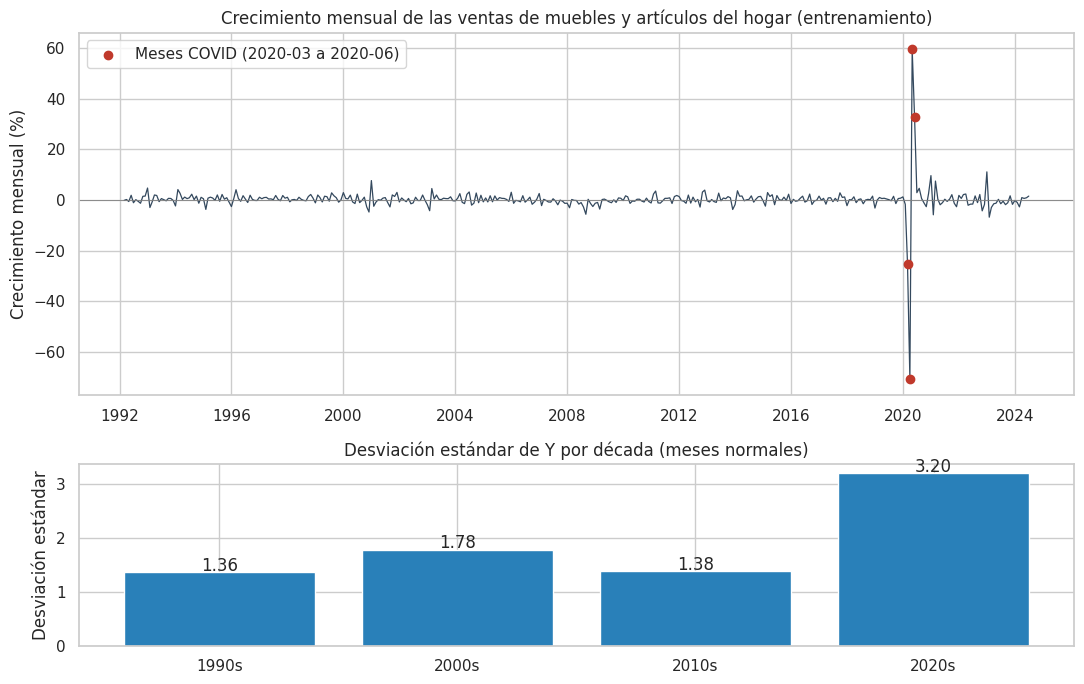
\includegraphics[width=\linewidth]{figuras/fig_B1_serie_tiempo.png}
  \caption{Crecimiento mensual de ventas de muebles (arriba) y desviación estándar por década en meses normales (abajo).}
  \label{fig:serie}
\end{figure}

\begin{figure}[!ht]
  \centering
  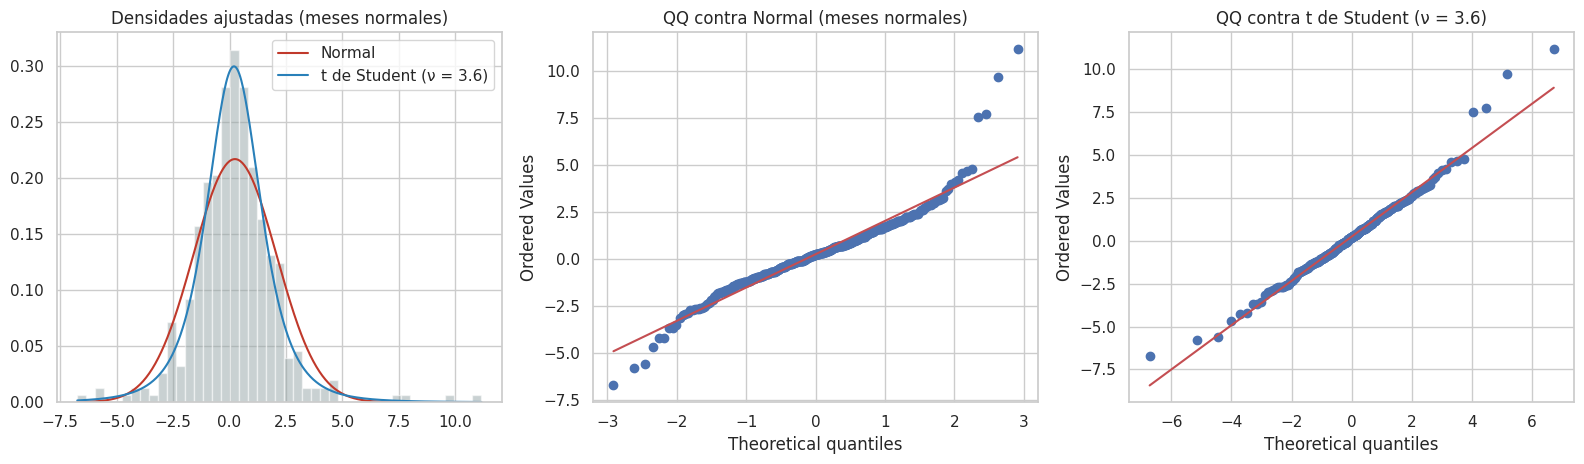
\includegraphics[width=\linewidth]{figuras/fig_B5_ajuste_distribuciones.png}
  \caption{Ajuste de densidad normal y \textit{t} de Student al crecimiento en meses normales.}
  \label{fig:dist}
\end{figure}

\begin{figure}[!ht]
  \centering
  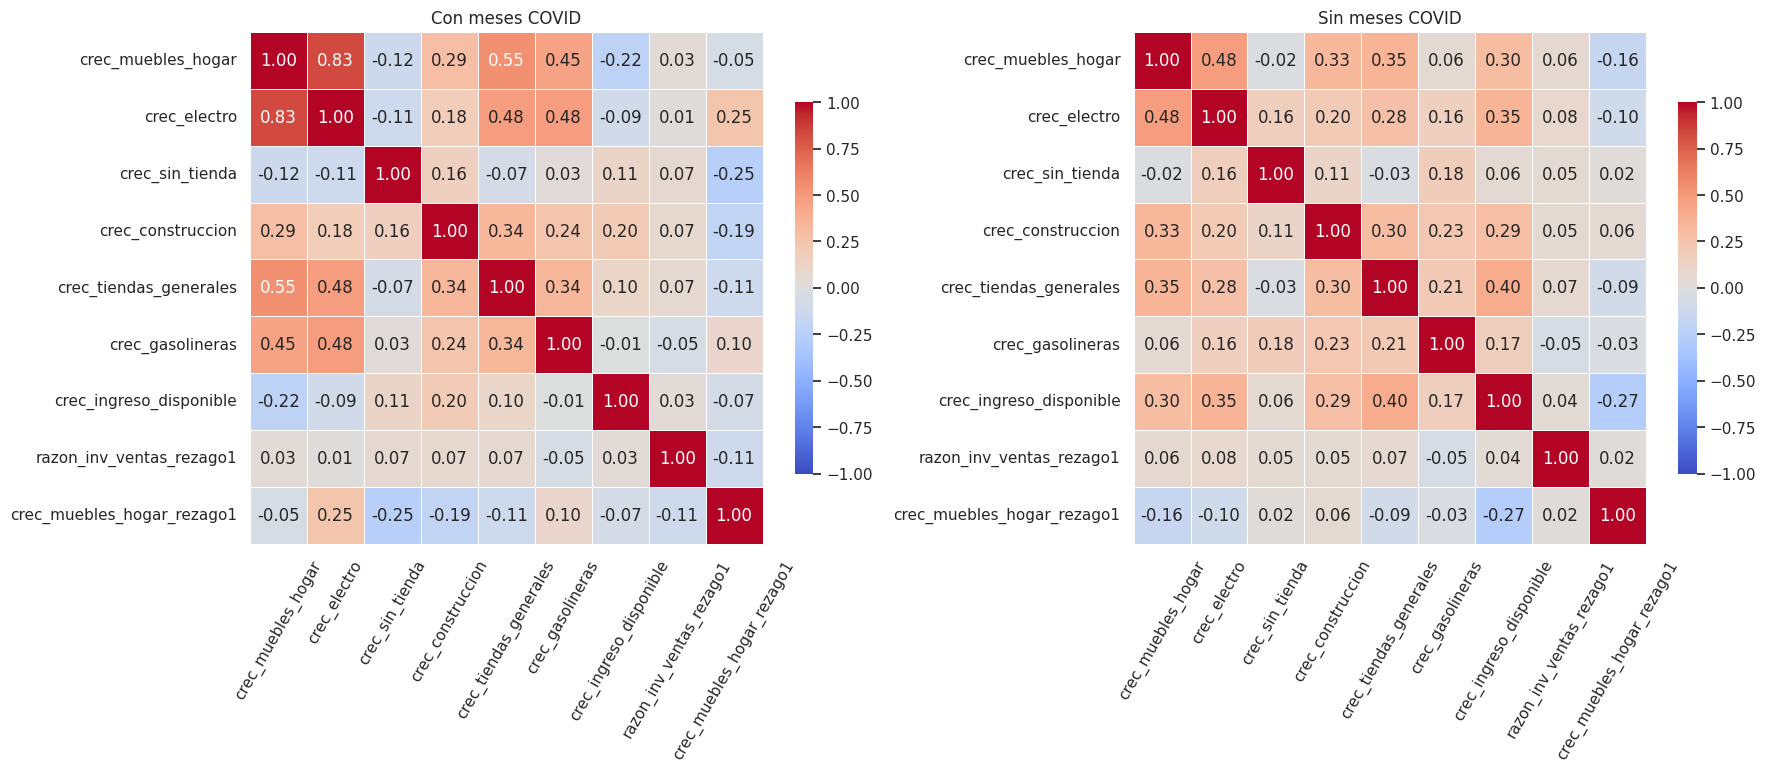
\includegraphics[width=\linewidth]{figuras/fig_B6_heatmap_correlaciones.png}
  \caption{Correlaciones de Pearson entre variables cuantitativas (con y sin meses COVID).}
  \label{fig:corr}
\end{figure}

\subsection{Multicolinealidad (VIF)}
En regresión múltiple, cuando dos explicativas se mueven juntas, el modelo puede ajustar bien pero las posteriores de $\beta_j$ se vuelven anchas y correlacionadas entre sí. El factor de inflación de la varianza cuantifica ese riesgo: $\mathrm{VIF}_j=1/(1-R_j^2)$, donde $R_j^2$ proviene de regresar $X_j$ contra las demás explicativas. Reglas prácticas sugieren VIF$<5$ \citep{gelman2008weakly}. En meses normales el máximo es 1.43, y con COVID incluido los valores siguen bajos: las categorías del comercio covarían en el sector, pero no de forma tan redundante como para impedir inferencia por separado sobre cada coeficiente.

\subsection{Especificación del modelo}
\begin{equation}
y_t = \beta_0 + \sum_{j=1}^{8}\beta_j z_{jt} + \varepsilon_t,\quad
\varepsilon_t \sim t_\nu(0,\sigma_t),
\label{eq:modelo}
\end{equation}
con $\sigma_t = \sigma\,\lambda_t\,\psi^{I(t\ge\text{jul-2020})}$, $\lambda_t=\kappa_m$ en mar.--jun.\ 2020 y $\lambda_t=1$ en el resto. Son 16 parámetros: intercepto, ocho coeficientes, $\sigma$, $\nu$, cuatro $\kappa_m$ y $\psi$. La \textit{t} robustece frente a colas pesadas \citep{lange1989}; los factores $\kappa_m$ siguen la idea de modelar la volatilidad pandémica \citep{lenza2022}; $\psi$ captura el aumento sostenido de volatilidad desde jul.\ 2020 visto en el EDA.

\subsection{Distribuciones a priori}
Los hiperparámetros combinan \textbf{orden de magnitud del EDA} y recomendaciones bibliográficas; no se ajustaron iterando hasta obtener una posterior deseada ni se elicitaron con un experto del sector. Sí se usó información legítima de escala: en meses normales $\mathrm{SD}(y)\approx 1.8$ puntos, acotando cuánto podría moverse $y$ si otra variable aumenta una desviación típica \citep{gelman2006prior,gelman2008weakly}.

En resumen: $\beta_j\sim\mathcal{N}(0,1)$ (solo 4.6\% de masa a priori con $|\beta_j|>2$); $\sigma\sim\mathrm{HN}(0,2)$ cubriendo valores desde ruido residual pequeño hasta la dispersión histórica; $\nu\sim\mathrm{Gamma}(2,0.1)$ siguiendo \citet{juarez2010} para grados de libertad de una \textit{t}; $\log\kappa_m\sim\mathrm{HN}(0,1)$ permitiendo meses COVID muy volátiles; $\log\psi\sim\mathcal{N}(0,1)$ con mediana en $\psi=1$ (sin cambio estructural a priori). El chequeo predictivo a priori (Fig.~\ref{fig:priors}) simula trayectorias de $y_t$: en meses normales las simulaciones se alinean con $\pm 2$ puntos, y en COVID admiten colas largas sin forzar la posterior.

\begin{figure}[!ht]
  \centering
  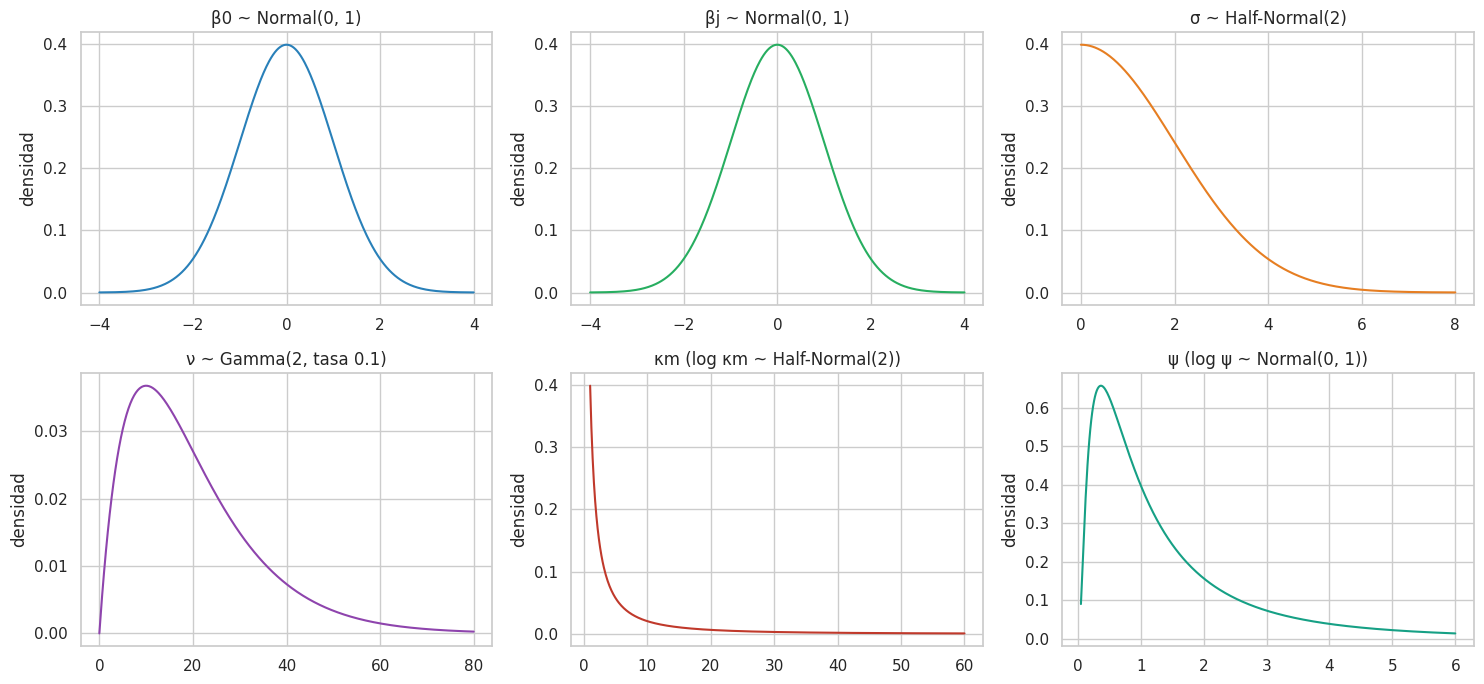
\includegraphics[width=\linewidth]{figuras/fig_C1_densidades_priors.png}
  \caption{Densidades a priori de parámetros principales.}
  \label{fig:priors}
\end{figure}

\subsection{Inferencia bayesiana (MCMC)}
No hay forma analítica para la posterior de 16 parámetros con escalas heterogéneas por mes. Implementamos Metropolis--Hastings aleatorio con propuesta multivariada normal. Durante el calentamiento se adapta la matriz de covarianza de la propuesta a la empírica de las iteraciones, escalada por $2.38^2/16$ para aproximar una tasa de aceptación del 23\% en regiones casi normales de la posterior \citep{roberts1997}. Después del quemado la propuesta queda fija, de modo que las muestras guardadas provienen de una cadena válida.

Corren \textbf{cuatro cadenas} independientes con 30\,000 iteraciones de quemado y 40\,000 de muestreo cada una (configuración de entrega en el cuaderno). Se exige $\hat R<1.01$ y ESS $\ge 2000$ en cada parámetro \citep{vehtari2021}; las trazas solapadas (Fig.~\ref{fig:trazas}) indican exploración conjunta del mismo modo posterior. La log-posterior y la regla de aceptación se detallan en el Apéndice~A.

\begin{figure}[!ht]
  \centering
  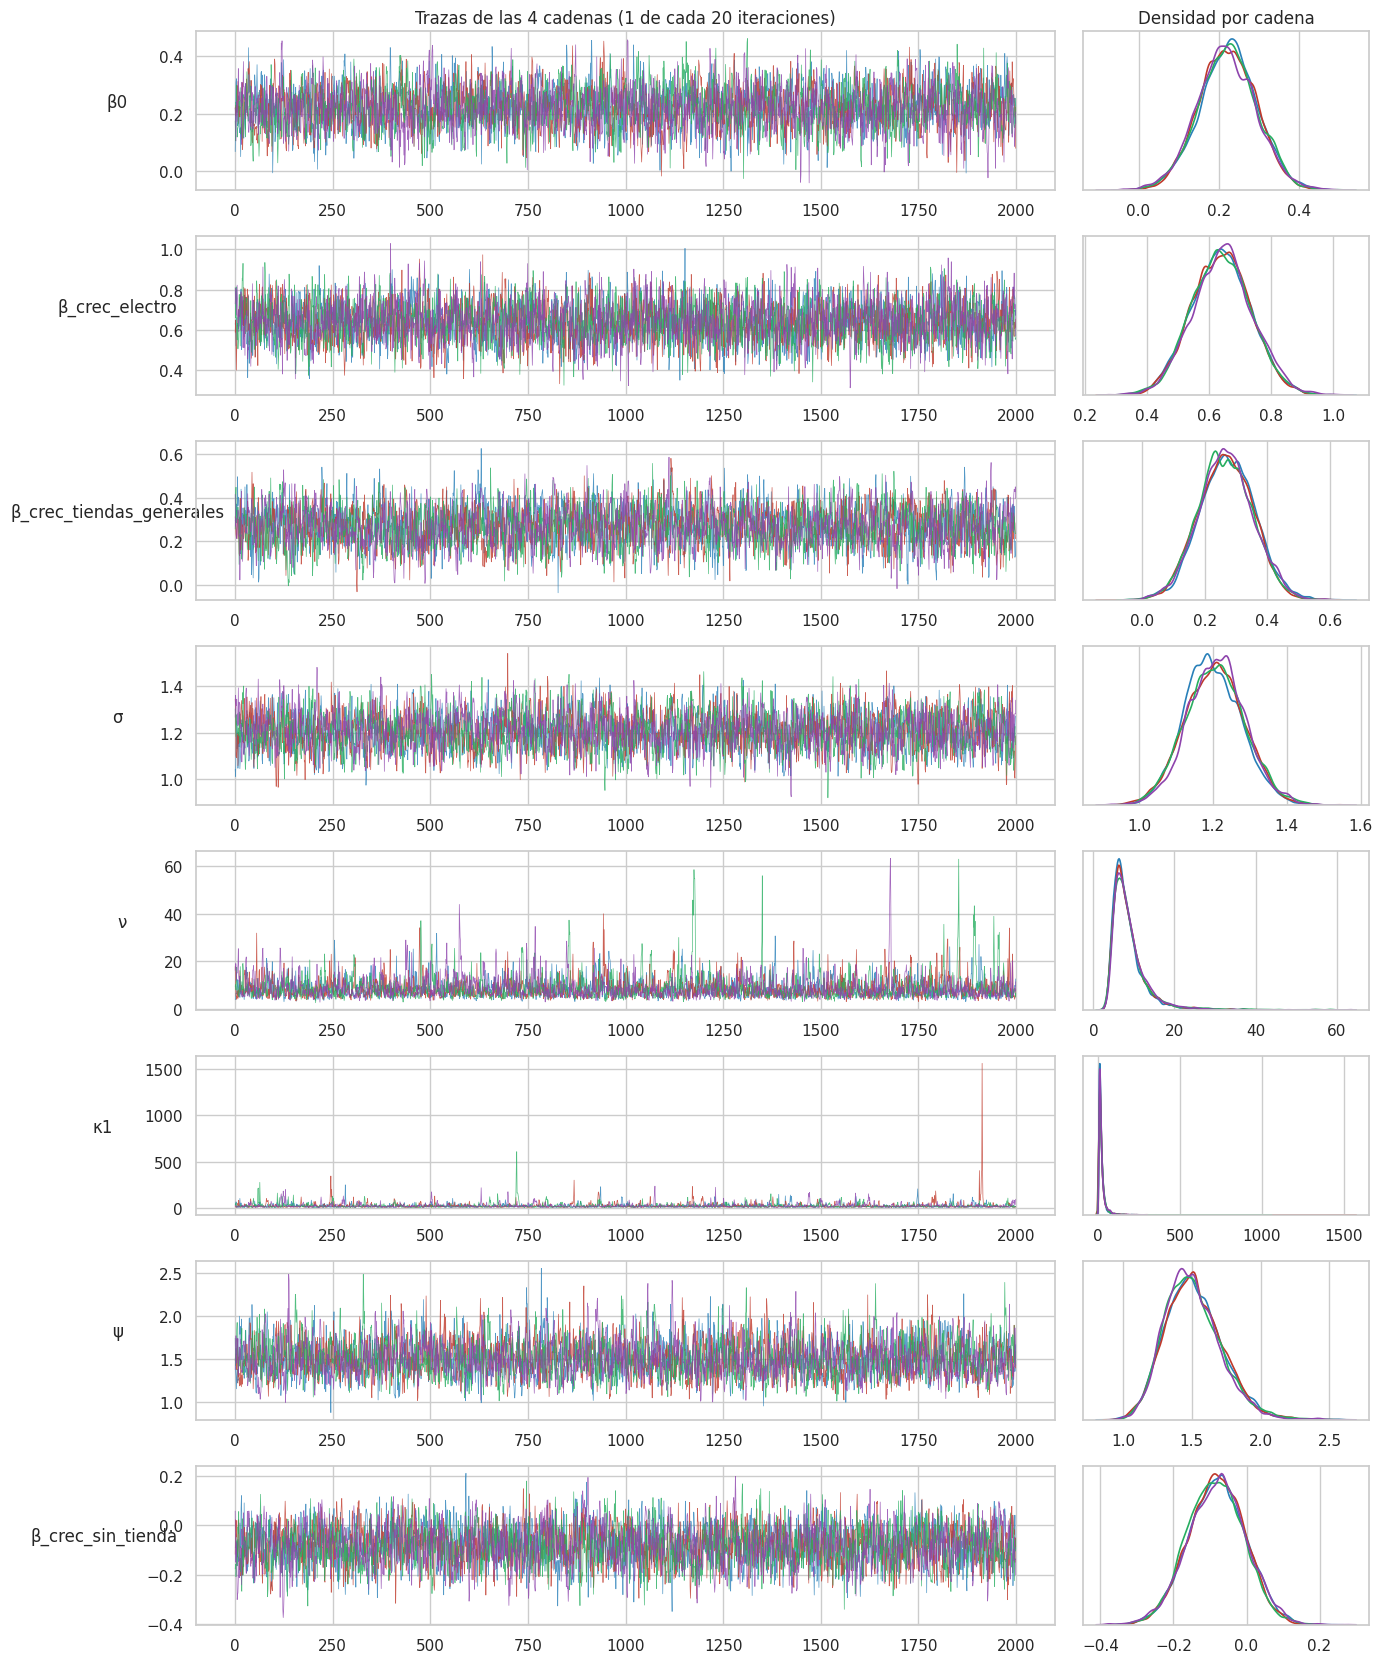
\includegraphics[width=\linewidth]{figuras/fig_D1_trazas.png}
  \caption{Trazas MCMC de parámetros seleccionados (cuatro cadenas).}
  \label{fig:trazas}
\end{figure}

\section{Resultados}
\subsection{Coeficientes y capacidad explicativa}
Las cadenas convergen ($\hat R$ máximo 1.004). La Tabla~\ref{tab:coef} resume medias posteriores e intervalos creíbles del 95\% de $\beta_j$ en variables estandarizadas (Fig.~\ref{fig:coef}): un coeficiente de 0.64 en electrónica significa que, cuando el crecimiento de esa categoría está una desviación por encima de su media, el crecimiento de muebles tiende a subir unos 0.64 puntos, \textbf{manteniendo constantes las demás variables del mes}.

Electrónica (+0.64), construcción (+0.40) y tiendas generales (+0.27) acompañan positivamente al sector; gasolineras muestran relación negativa débil ($-0.18$) con intervalo que apenas excluye cero---la interpretamos con cautela por falta de mecanismo directo claro. Ingreso, canal sin tienda, razón inventarios/ventas y rezago de muebles no muestran evidencia contundente (IC 95\% incluyen 0), aunque el rezago concentra 95.5\% de probabilidad posterior bajo cero.

El $R^2$ bayesiano medio fue 0.31 en meses normales del entrenamiento y 0.05 en prueba: el modelo captura co-movimiento del sector en la historia, pero \textbf{no explica la mayor parte} de la variación mes a mes en datos nuevos. Por eso no esperamos dominar la media histórica en RMSE; el valor está en la distribución predictiva.

\begin{table}[!ht]
\centering
\small
\begin{tabular}{lrr}
\hline
\textbf{Variable} & \textbf{Media post.} & \textbf{IC 95\%} \\
\hline
Electrónica y electrodomésticos & 0.640 & 0.456 -- 0.829 \\
Materiales de construcción & 0.401 & 0.242 -- 0.568 \\
Tiendas de mercancía general & 0.268 & 0.098 -- 0.437 \\
Estaciones de gasolina & $-0.176$ & $-0.331$ -- $-0.025$ \\
Ingreso disponible & 0.112 & $-0.091$ -- 0.327 \\
Ventas sin tienda & $-0.082$ & $-0.235$ -- 0.069 \\
Razón inventarios/ventas & $-0.001$ & $-0.161$ -- 0.157 \\
Crecimiento muebles (rezago 1) & $-0.122$ & $-0.273$ -- 0.017 \\
\hline
\end{tabular}
\caption{Posterior de coeficientes de regresión (escala estandarizada).}
\label{tab:coef}
\end{table}

\subsection{Volatilidad, colas y episodios extremos}
La mediana posterior de $\nu$ es 7.6: hay más probabilidad en movimientos grandes que bajo una normal con la misma escala. La escala basal $\sigma$ y el factor $\psi$ describen el \textbf{régimen post-2020}: $\psi$ con mediana 1.50 y probabilidad 99.9\% de superar 1 implica que la desviación típica del error pasó de unos 1.4 a 2.1 puntos de crecimiento. Los $\kappa_m$ de marzo--junio de 2020 tienen medianas entre 15 y 35, absorbiendo picos sin arrastrar $\beta_j$ hacia valores irreales (Fig.~\ref{fig:sigmapsi}). En términos de inventario, planificar con la volatilidad pre-2020 sería optimista frente al comportamiento reciente del sector.

\begin{figure}[!ht]
  \centering
  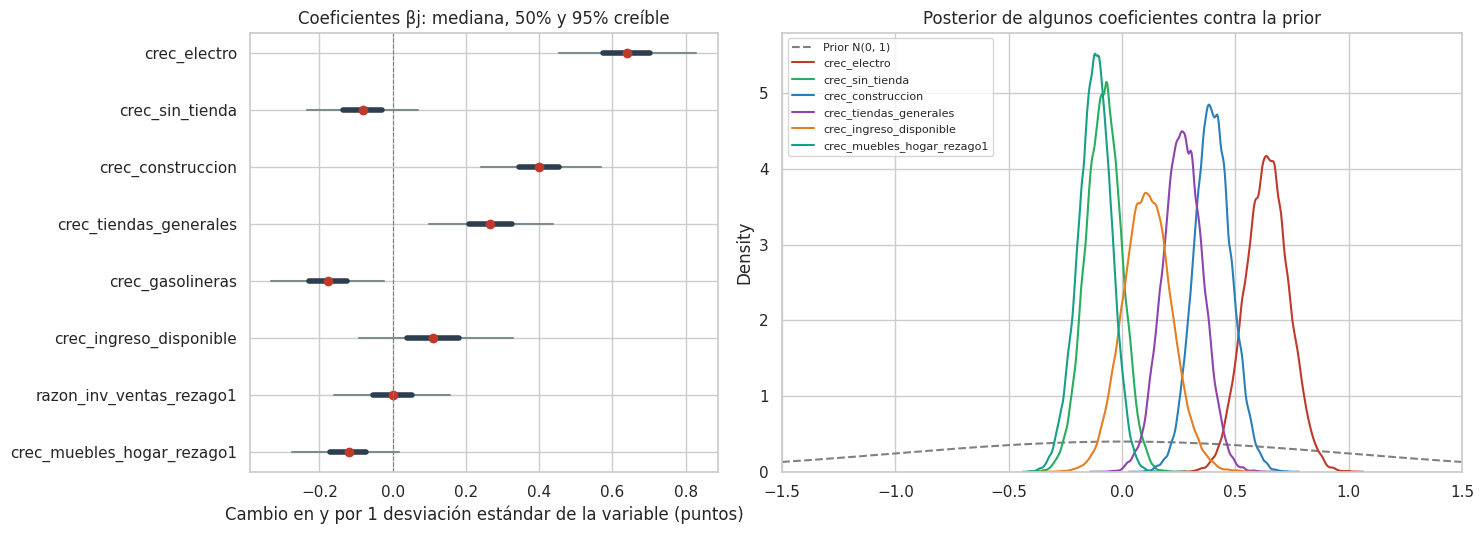
\includegraphics[width=\linewidth]{figuras/fig_D3_coeficientes.png}
  \caption{Mediana e intervalos creíbles de coeficientes; panel derecho: prior vs.\ posterior.}
  \label{fig:coef}
\end{figure}

\begin{figure}[!ht]
  \centering
  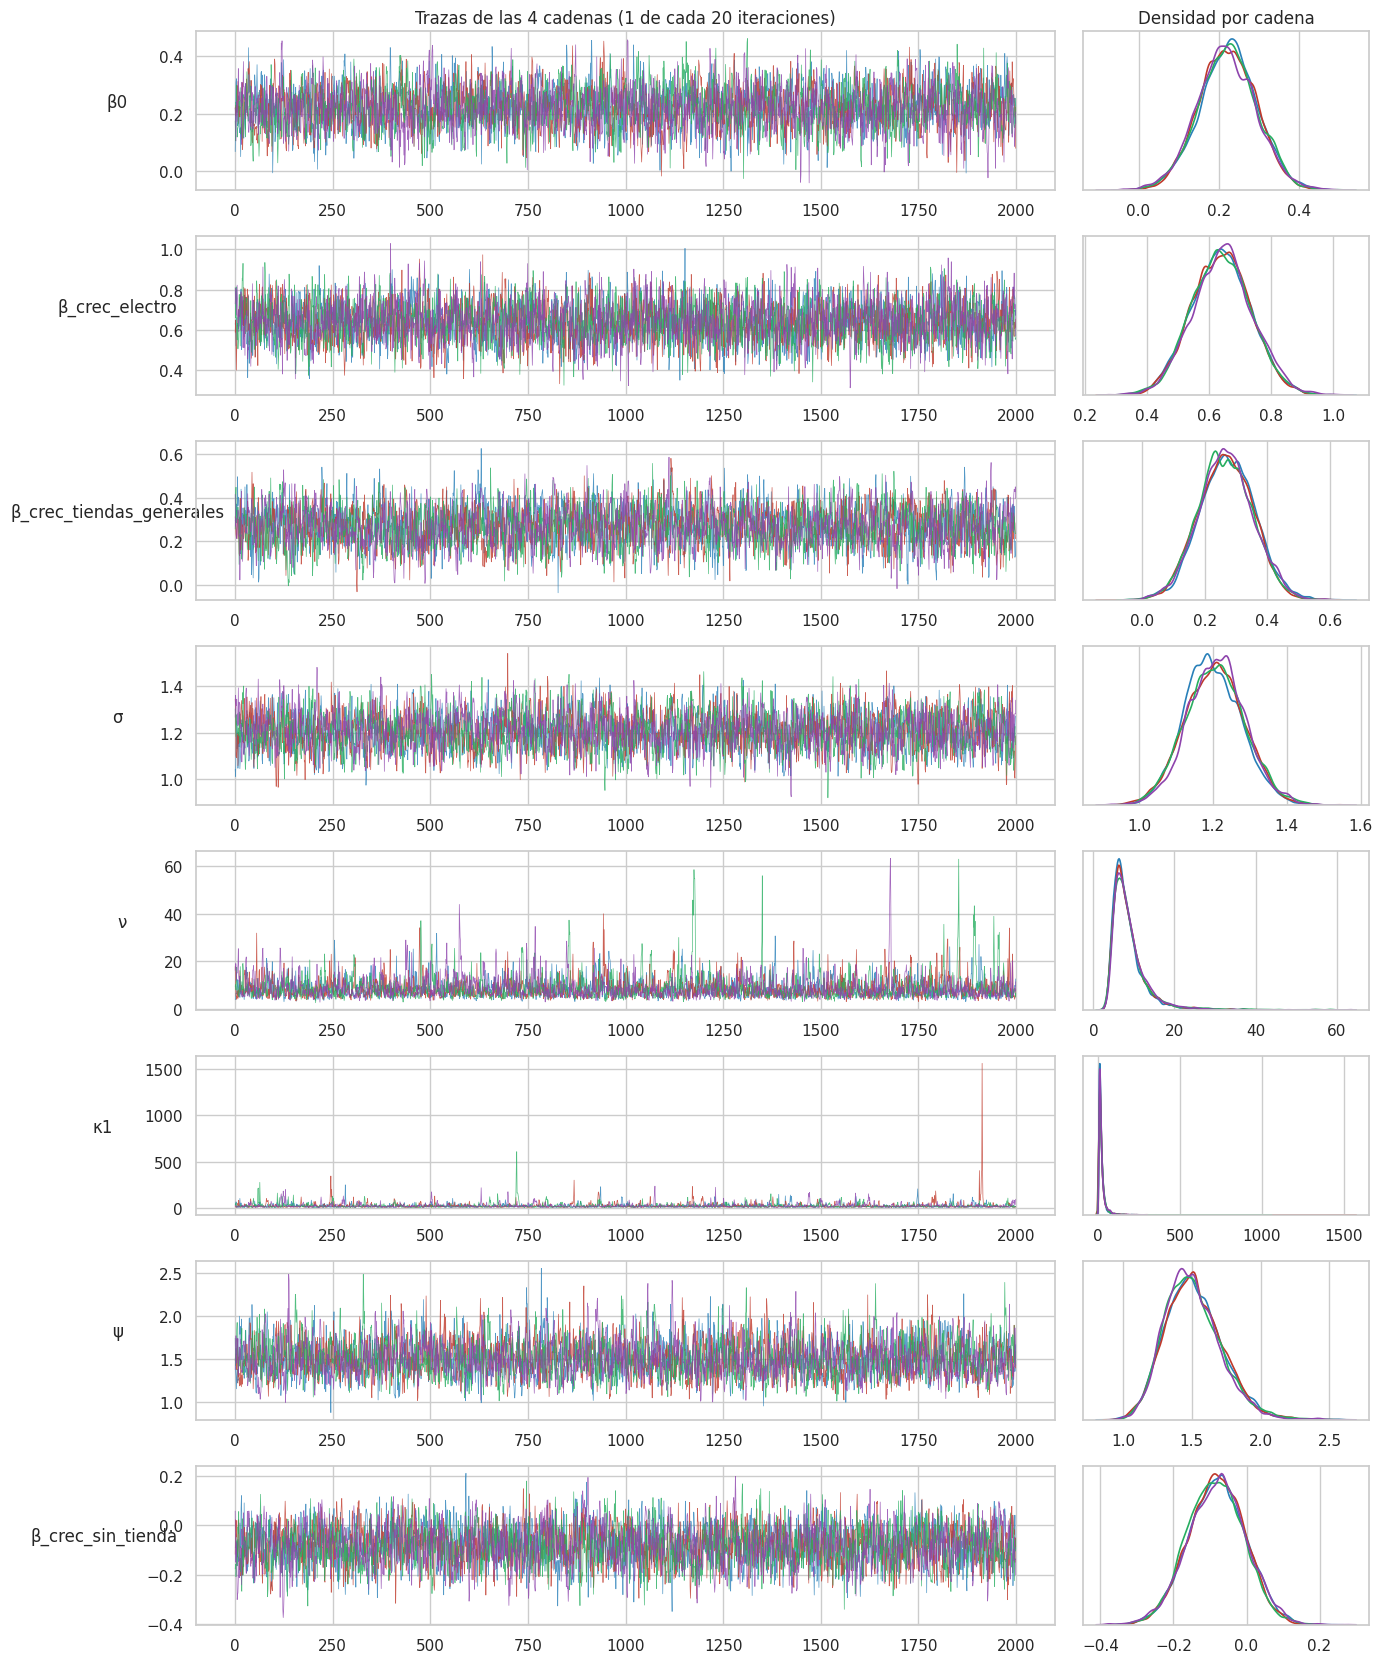
\includegraphics[width=\linewidth]{figuras/fig_D4_sigma_nu_psi.png}
  \caption{Posterior de $\sigma$, $\nu$ y $\psi$ frente a priors.}
  \label{fig:sigmapsi}
\end{figure}

\subsection{Validación en el conjunto de prueba}
Comparamos el modelo bayesiano con referencias que una empresa podría usar sin regresión: la \textbf{media histórica} del crecimiento, la \textbf{persistencia} (repetir el cambio del mes anterior) y una \textbf{\textit{t} marginal} ajustada solo a la historia de $y$ sin factores de pandemia.

En predicción puntual el modelo \textbf{no supera} la media histórica (RMSE 2.04 vs.\ 2.02); la persistencia es claramente peor (3.28). La ventaja aparece en los \textbf{intervalos predictivos}: el 90\% cubrió 23/24 meses (solo diciembre de 2024 quedó fuera), con ancho medio 6.9 puntos frente a 9.5 de la \textit{t} simple (Tabla~\ref{tab:metricas}, Fig.~\ref{fig:valid}). Intervalos más angostos con cobertura similar reducen sobre-stock innecesario si la empresa usa el techo del intervalo como escenario de stress. CRPS 1.15 vs.\ 1.17 indica una ligera mejora en la distribución completa, aunque con 24 meses no es concluyente. Coberturas del 80\% y 50\% fueron 79\% y 37.5\%; la del 50\% puede reflejar azar muestral.

\begin{table}[!ht]
\centering
\small
\begin{tabular}{lcccc}
\hline
\textbf{Método} & RMSE & CRPS & Ancho 90\% & Cob. 90\% \\
\hline
Modelo bayesiano & 2.04 & 1.15 & 6.9 & 0.96 \\
\textit{t} solo en $y$ & 2.04 & 1.17 & 9.5 & 0.96 \\
Media histórica & 2.02 & --- & --- & --- \\
Persistencia & 3.28 & --- & --- & --- \\
\hline
\end{tabular}
\caption{Métricas en conjunto de prueba (crecimiento mensual, puntos porcentuales).}
\label{tab:metricas}
\end{table}

\begin{figure}[!ht]
  \centering
  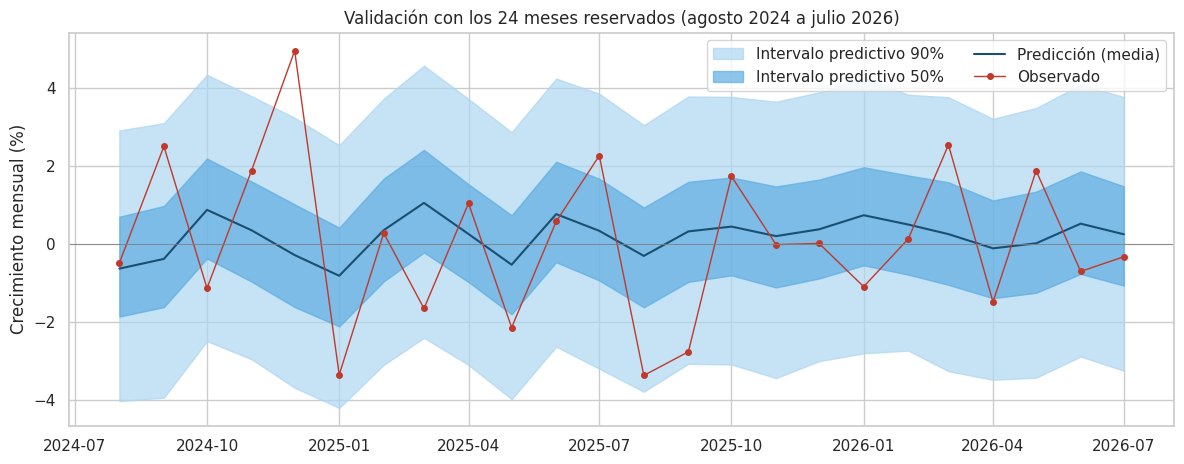
\includegraphics[width=\linewidth]{figuras/fig_E1_validacion_prueba.png}
  \caption{Crecimiento observado y predicho en prueba, con intervalos predictivos 50\% y 90\%.}
  \label{fig:valid}
\end{figure}

\subsection{Rango sectorial para el mes siguiente}
Para pasar de crecimiento a \textbf{nivel de ventas} usamos $V_t = V_{t-1}\exp(g_t/100)$, con $V_{t-1}$ observado. En los 24 meses de prueba los intervalos creíbles en millones USD contendieron las ventas observadas en la misma proporción que los intervalos en $y_t$.

Para \textbf{agosto de 2026} (posterior a julio, con ventas de julio en 10\,537 millones USD) el cambio mensual del sector estaría entre $-3.8\%$ y $+4.9\%$ con probabilidad 90\%, equivalente a 10\,134--11\,050 millones (Fig.~\ref{fig:inventario}). La mediana predictiva ronda 10\,542 millones. El intervalo es algo más ancho que en prueba porque, en el cuaderno, las covariables de agosto se promedian sobre escenarios posibles desde julio de 2020 (no se conocen al cerrar julio). Ese mes no tiene dato oficial aún, por lo que el rango es \textbf{prospectivo}, no validado.

\begin{figure}[!ht]
  \centering
  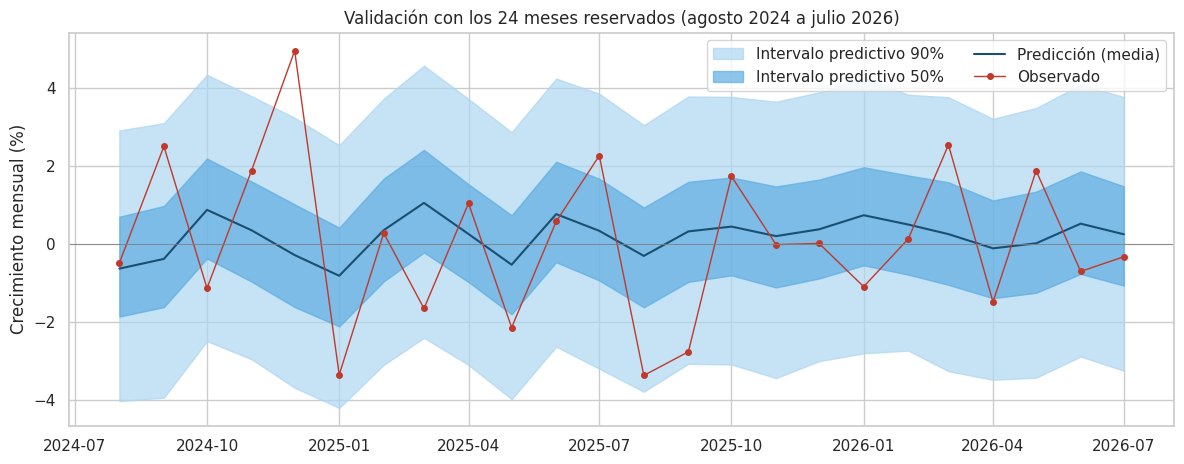
\includegraphics[width=\linewidth]{figuras/fig_F1_rango_inventario.png}
  \caption{Ventas en prueba con intervalo 90\% y distribución predictiva de ventas (ago.\ 2026).}
  \label{fig:inventario}
\end{figure}

\section{Discusión}
La pregunta del proyecto admite dos respuestas. Primero, \textbf{escala de la variación}: en meses tranquilos el cambio absoluto del sector suele ser menor que 2 puntos, pero desde mediados de 2020 la volatilidad se duplicó---cualquier plan micro que ignore ese régimen arrastra riesgo. Segundo, \textbf{predictibilidad puntual limitada}: aun con covariables del mismo mes, el $R^2$ en prueba es bajo; el entregable útil es la distribución del cambio y del nivel de ventas, no una cifra exacta.

\subsection{De la referencia macro a decisiones micro}
Ilustramos un flujo que una comercializadora en EE.\ UU.\ podría seguir \textbf{sin sustituir} su pronóstico interno, sino acotándolo con el sector (Tabla~\ref{tab:aplicacion}).

\textbf{Paso 1---Escenario sectorial.} Tomar del modelo la mediana y el intervalo 90\% de ventas del mes siguiente en millones USD del mercado nacional (p.\,ej.\ agosto 2026: mediana 10\,542; piso 10\,134; techo 11\,050).

\textbf{Paso 2---Traducción a la firma.} Si la empresa vende una fracción $s$ del mercado o usa su propia serie desestacionalizada, proyecta ventas propias $V^{\mathrm{micro}} \approx s \cdot V^{\mathrm{macro}}$ o aplica un factor de desviación histórica $k$ (su crecimiento suele ser 1.2 veces el del sector). El intervalo macro se escala: ancho relativo $\pm 3.9\%$ / $+4.9\%$ se traslada a dólares de la empresa.

\textbf{Paso 3---Inventario de seguridad.} La brecha entre mediana y percentil 95 (unos 508 millones a nivel sector, $\approx$4.8\% sobre la mediana) funciona como \textbf{colchón orientativo} frente a meses fuertes. Compras compara esa holgura con el costo de faltante y el lead time; finanzas contrasta el escenario piso ($-3.9\%$) con inventario actual para detectar riesgo de sobrestock.

\textbf{Paso 4---Coordinación interna.} Compras, comercial y finanzas discuten con el mismo triplete (mediana, piso, techo) en lugar de tres puntos distintos. El modelo bayesiano permite además preguntas probabilísticas (p.\,ej.\ 18\% de caída mayor a 2\% en el cuaderno), útiles para políticas de servicio.

\begin{table}[!ht]
\centering
\small
\begin{tabular}{lrr}
\hline
\textbf{Escenario (ago.\ 2026)} & \textbf{Ventas sector (M USD)} & \textbf{vs.\ mediana} \\
\hline
Percentil 5 (piso 90\%) & 10\,134 & $-3.9\%$ \\
Mediana predictiva & 10\,542 & --- \\
Percentil 95 (techo 90\%) & 11\,050 & $+4.8\%$ \\
Ventas jul.\ 2026 (base) & 10\,537 & --- \\
\hline
\end{tabular}
\caption{Ejemplo de referencia macro para el sector. La empresa escala a su volumen $s$ o ajusta con su factor $k$ histórico.}
\label{tab:aplicacion}
\end{table}

\textbf{Qué no hace esta referencia.} No estima demanda por SKU ni precio; no incorpora promociones ni competencia local. El agregado \textbf{suaviza} idiosincrasias: una tienda puede caer cuando el sector sube. Las covariables miden \textbf{asociación contemporánea}, no causalidad. Con solo 24 meses de prueba, la cobertura del 90\% es alentadora pero no es garantía estadística fuerte. Ante un choque nuevo tipo 2020, el rango vigente quedaría corto hasta reestimar $\kappa_m$ y $\psi$.

\subsection{Síntesis metodológica}
Conservar COVID y $\psi$ estrecha intervalos sin perder cobertura frente a borrar 2020 o ignorar el cambio de régimen. La \textit{t} y los factores de escala son coherentes con el EDA (colas y heteroscedasticidad). Los priors débiles evitan dominar con supuestos fuertes, dejando que los datos hablen en $\beta_j$ y en volatilidad.

\section{CONCLUSIONES}
Respondimos cuánto puede variar mensualmente el sector de muebles y artículos del hogar en EE.\ UU.\ y con qué incertidumbre. En meses normales el cambio típico es moderado, pero la volatilidad desde julio de 2020 más que duplicó la de la era pre-pandemia; ignorar ese hecho llevaría a rangos de inventario demasiado estrechos en el presente.

Electrónica, construcción y tiendas generales se mueven junto con muebles; ingreso, canal online e inventarios del canal no mostraron relaciones claras. El poder predictivo puntual es limitado ($R^2$ bajo en prueba; RMSE similar a la media histórica), pero los \textbf{intervalos bayesianos del 90\%} cubrieron 23 de 24 meses y fueron más angostos que una alternativa sin factores COVID/$\psi$.

Para agosto de 2026 el sector podría situarse entre 10\,134 y 11\,050 millones USD al 90\%, con mediana cerca de 10\,542 millones---cifras que una comercializadora puede escalar a su volumen para fijar techo de compra, piso de cobertura e inventario de seguridad, siempre contrastando con su historial micro.

El aporte central es un \textbf{lenguaje común de incertidumbre} entre áreas de la empresa, anclado en datos macro públicos y reproducible con \texttt{codigo\_final\_vf.ipynb}. No reemplaza el pronóstico interno; lo complementa con un escenario sectorial calibrado.

\onecolumn
\section*{APÉNDICE MATEMÁTICO}
\justifying

\subsection*{A.1 Posterior y log-posterior}
Por el teorema de Bayes,
$p(\boldsymbol{\theta}\mid\mathbf{y})\propto \big[\prod_{t=1}^{389} t_\nu(y_t\mid\mu_t,\sigma_t)\big]\,p(\boldsymbol{\theta})$,
con $\boldsymbol{\theta}=(\beta_0,\ldots,\beta_8,\sigma,\nu,\kappa_1,\ldots,\kappa_4,\psi)$ y $\mu_t=\beta_0+\sum_j\beta_j z_{jt}$. Se muestrean $\log\sigma$, $\log\nu$, $u_m=\log\kappa_m\ge 0$ y $\log\psi$, añadiendo jacobianos donde corresponde. La log-posterior incluye la suma de log-verosimilitudes \textit{t}, priors de $\beta_j$ normales, half-normal sobre escalas y término $2\log\nu-0.1\nu$ para $\nu$.

\subsection*{A.2 Razón de aceptación (MH)}
Con propuesta $q(\boldsymbol{\theta}^*\mid\boldsymbol{\theta})$ simétrica,
$\alpha(\boldsymbol{\theta},\boldsymbol{\theta}^*)=\min\{1,\exp[\log p(\boldsymbol{\theta}^*\mid\mathbf{y})-\log p(\boldsymbol{\theta}\mid\mathbf{y})]\}$.
Tras calentamiento, $\boldsymbol{\Sigma}=2.38^2/16\,\widehat{\mathrm{Cov}}(\boldsymbol{\theta})$ permanece fija.

\subsection*{A.3 Diagnósticos}
$\hat R=\sqrt{\frac{n-1}{n}W+\frac{1}{n}B}\big/ W$ con varianzas entre e intra cadenas \citep{vehtari2021}. ESS $=mn/(1+2\sum_k\hat\rho_k)$ con corte en autocorrelaciones negativas consecutivas.

\subsection*{A.4 Predicción, ventas en nivel y uso operativo}
Para cada extracción $\boldsymbol{\theta}^{(s)}$ y mes nuevo con covariables $z^*$, se simula $y_*^{(s)}$ de la \textit{t} predictiva con escala $\sigma^{(s)}(\psi^{(s)})^{I(\cdot\ge\text{jul-2020})}$ y factores $\kappa_m$ si aplica. Los cuantiles de $\{y_*^{(s)}\}$ definen intervalos de crecimiento; las ventas en millones son $V_*^{(s)}=V_{t-1}\exp(y_*^{(s)}/100)$. Cuando $z^*$ no se conoce (mes futuro), el cuaderno muestrea $z^*$ de meses observados desde jul.\ 2020, propagando incertidumbre adicional al rango macro que luego la empresa escala a su nivel micro. El $R^2$ bayesiano por extracción es $\mathrm{Var}(\mu_t)/[\mathrm{Var}(\mu_t)+\mathrm{Var}(y_t-\mu_t)]$ en meses normales del entrenamiento.

\twocolumn
\bibliographystyle{apalike}
\bibliography{Bibliografia}

\end{document}
